\documentclass[11pt,a4paper]{article}
\usepackage[utf8]{inputenc}
\usepackage[german]{babel}
\usepackage{amsmath}
\usepackage{amsfonts}
\usepackage{subfig}
\usepackage{amssymb}
\usepackage{siunitx,physics}
\usepackage{mathtools}
\usepackage{graphicx}
%\usepackage{Here}
\usepackage[version=4]{mhchem}
\usepackage{url}
\usepackage{setspace}
\usepackage[left=2.5cm,right=2.5cm,top=2.5cm,bottom=2cm]{geometry}
[biblography=totocnumbered]
\usepackage{fancyhdr}
\usepackage{scrextend}
\usepackage{hyperref}
\pagenumbering{gobble}

\makeatletter
\newcommand\bigcdot{\mathpalette\bigcdot@{.5}}
\newcommand\bigcdot@[2]{\mathbin{\vcenter{\hbox{\scalebox{#2}{$\m@th#1\bullet$}}}}}
\makeatother

\makeatletter
%\renewcommand*\bib@heading{%
%  \subsection*{}%
%  \@mkboth{\refname}{\refname}}
%\makeatother
\numberwithin{equation}{section}
\numberwithin{figure}{section}

\renewcommand{\labelitemii}{\labelitemfont$\vartriangleright$}
\begin{document}\\
\begin{addmargin}[25pt]{0pt}
\begin{itemize}
    \item Zugversuch
    \begin{itemize}
        \item uniaxiale Dehnung entlang der Achse eines elastischen Stabs
        \item Stab wird länger entlang Kraftwirkung und schmaler senkrecht zur Kraft
        \item Dehnung entlang der Kraft ist definiert als $\epsilon = \frac{\Delta l}{l_0}$
        \item $\Delta l :=$ Längenänderung bei angelegter Kraft; $l_0 :=$ ursprüngliche Länge des Stabs
        \item Spannung $\sigma$ ergibt sich aus Elastizitätsmodul $E$ und Dehnung $\epsilon$: $\sigma = E\cdot\epsilon$ 
        \item Spannung ist ebenfalls über angelegte Kraft $F$ und ursprüngliche Querschnittsfläche $A_0$ definiert: $\sigma = \frac{F}{A_0}$
    \end{itemize}
    \item Druckversuch
    \begin{itemize}
        \item wie Zugversuch aber Stauchung anstatt Dehnung 
        \item Unterschied: Kraft hat anderes Vorzeichen
    \end{itemize}
    \item Scherversuch
    \begin{itemize}
        \item Kraft wirkt nicht mehr senkrecht auf Oberfläche sondern parallel
        \item Scherspannung $\tau$ ist analog zu Spannung beim Zugversuch definiert: $\tau = \frac{F}{A_0}$
        \item Scherdehnung $\gamma$ ist der Tangens des Winkels $\theta$ um den sich Probe verdreht: $\gamma = \tan\theta$
        \item Es gilt wieder: $\tau = G\cdot\gamma$, dabei ist $G$ der Schubmodul
    \end{itemize}
    \item Torsionsversuch
    \begin{itemize}
        \item analog zu Scherversuch aber die betrachtete Verdrehung ist anders
        \item es wird Torsionsmoment angelegt wodurch der Körper um seine eigene Achse eingedreht wird
    \end{itemize}
\end{itemize}
Alle Versuche sind nochmal in Abbildung \ref{fig:Modulnversuche} visualisiert

\begin{figure}[h]
    \centering
    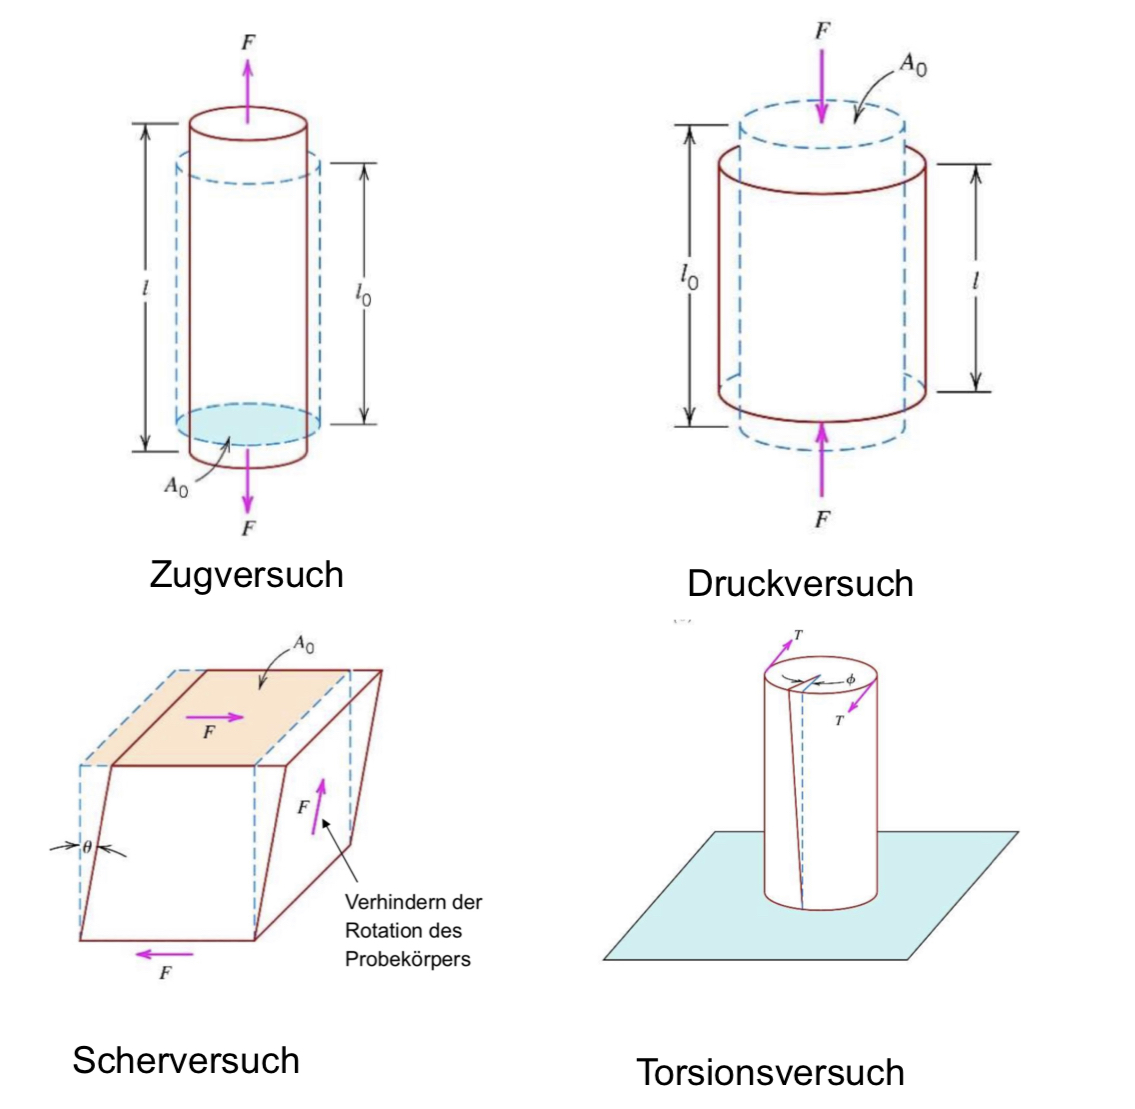
\includegraphics[width = 0.8\textwidth]{images/Materialwissenschaften/Modulnversuche.jpeg}
    \caption{Die 4 verschiedenen Versuche zur Bestimmung des Elastizitätsmoduls und des Schubmoduls visualisiert}
    \label{fig:Modulnversuche}
\end{figure}
\end{addmargin} 


\end{document}